\documentclass{beamer}
\usepackage{etex} % fixes new-dimension error
\usepackage{lmodern}
\usepackage[T1]{fontenc}
\usepackage{mathtools}
%%%%%%%%%%%%% Macros
%%%% Categories
\newcommand{\catfont}[1]{\mathsf{#1}}
\newcommand{\cop}{\catfont{op}}
\newcommand{\Law}{\catfont{Law}}
\newcommand{\catV}{\catfont{V}}
\newcommand{\catX}{\catfont{X}}
\newcommand{\catC}{\catfont{C}}
\newcommand{\catD}{\catfont{D}}
\newcommand{\catA}{\catfont{A}}
\newcommand{\catB}{\catfont{B}}
\newcommand{\catI}{\catfont{I}}
\newcommand{\Set}{\catfont{Set}}
\newcommand{\Top}{\catfont{Top}}
\newcommand{\Pos}{\catfont{Pos}}
\newcommand{\Inj}{\catfont{Inj}}
\newcommand{\Det}{\catfont{RMhat}}
\newcommand{\CoAlg}[1]{\catfont{CoAlg}\left (#1 \right )}
\newcommand{\Mon}{\catfont{Mon}}
\newcommand{\Mnd}{\catfont{Mnd}(\catC)}
\newcommand{\SMnd}{\catfont{Mnd}(\Set)}
\newcommand{\CLat}{\catfont{CLat}}
\newcommand{\Stone}{\catfont{Stone}}
\newcommand{\Spectral}{\catfont{Spectral}}
\newcommand{\CompHaus}{\catfont{CompHaus}}
\newcommand{\Subs}[2]{\catfont{Sub}_{}}
\newcommand{\Cone}{\catfont{Cone}}
\newcommand{\StComp}{\catfont{StablyComp}}
\newcommand{\PosC}{\catfont{PosComp}}
\newcommand{\Haus}{\catfont{Haus}}
\newcommand{\Meas}{\catfont{Meas}}
\newcommand{\Ord}{\catfont{Ord}}
\newcommand{\EndoC}{[\catC,\catC]}
%% General functors
\newcommand{\funfont}[1]{#1}
\newcommand{\funF}{\funfont{F}}
\newcommand{\funU}{\funfont{U}}
\newcommand{\funG}{\funfont{G}}
\newcommand{\funT}{\funfont{T}}
\newcommand{\funI}{\funfont{I}}
%% Particular kinds of functors
\newcommand{\sfunfont}[1]{\mathrm{#1}}
\newcommand{\Pow}{\sfunfont{P}}
\newcommand{\Dist}{\sfunfont{D}}
\newcommand{\Maybe}{\sfunfont{M}}
\newcommand{\List}{\sfunfont{L}}
\newcommand{\UForg}{\sfunfont{U}}
\newcommand{\Forg}[1]{\sfunfont{U}_{#1}}
\newcommand{\Id}{\sfunfont{Id}}
\newcommand{\Vie}{\sfunfont{V}}
\newcommand{\Disc}{\funfont{D}}
\newcommand{\Weight}{\sfunfont{W}}
\newcommand{\homf}{\sfunfont{hom}}
\newcommand{\Yoneda}{\sfunfont{Y}}
%% Diagram functors
\newcommand{\Diag}{\mathscr{D}}
\newcommand{\KDiag}{\mathscr{K}}
\newcommand{\LDiag}{\mathscr{L}}
%% Monads
\newcommand{\monadfont}[1]{\mathbb{#1}}
\newcommand{\monadT}{\monadfont{T}}
\newcommand{\monadS}{\monadfont{S}}
\newcommand{\monadU}{\monadfont{U}}
\newcommand{\monadH}{\monadfont{H}}
\newcommand{\str}{\mathrm{str}}
%% Adjunctions
\newcommand\adjunct[2]{\xymatrix@=8ex{\ar@{}[r]|{\top}\ar@<1mm>@/^2mm/[r]^{{#2}}
& \ar@<1mm>@/^2mm/[l]^{{#1}}}}
\newcommand\adjunctop[2]{\xymatrix@=8ex{\ar@{}[r]|{\bot}\ar@<1mm>@/^2mm/[r]^{{#2}}
& \ar@<1mm>@/^2mm/[l]^{{#1}}}}
%% Retractions
\newcommand\retract[2]{\xymatrix@=8ex{\ar@{}[r]|{}\ar@<1mm>@/^2mm/@{^{(}->}[r]^{{#2}}
& \ar@<1mm>@/^2mm/@{->>}[l]^{{#1}}}}
%% Limits
\newcommand{\pv}[2]{\langle #1, #2 \rangle}
\newcommand{\limt}{\mathrm{lim}}
\newcommand{\pullbackcorner}[1][dr]{\save*!/#1+1.2pc/#1:(1,-1)@^{|-}\restore}
\newcommand{\pushoutcorner}[1][dr]{\save*!/#1-1.2pc/#1:(-1,1)@^{|-}\restore}
%% Colimits
\newcommand{\colim}{\mathrm{colim}}
\newcommand{\inl}{\mathrm{inl}}
\newcommand{\inr}{\mathrm{inr}}
%% Distributive categories
\newcommand{\distr}{\mathrm{dist}}
\newcommand{\undistr}{\mathrm{undist}}
%% Closedness
\newcommand{\curry}[1]{\mathrm{curry}{#1}}
\newcommand{\app}{\mathrm{app}}
%% Misc. operations
\newcommand{\const}[1]{\underline{#1}}
\newcommand{\comp}{\cdot}
\newcommand{\id}{\mathrm{id}}
%% Factorisations
\newcommand{\EClass}{E}
\newcommand{\MClass}{M}
\newcommand{\MConeClass}{\mathcal{M}}
%%%%%%%%%%%%%%%% End of Categorical Stuff

%%%% Misc
%% Operations
\newcommand{\blank}{\, - \,}
\newcommand{\sem}[1]{\llbracket #1 \rrbracket}
\newcommand{\closure}[1]{\overline{#1}}
\DeclareMathOperator{\img}{\mathrm{im}}
\DeclareMathOperator{\dom}{\mathrm{dom}}
\DeclareMathOperator{\codom}{\mathrm{codom}}
%% Sets of numbers
\newcommand{\Nats}{\mathbb{N}}
\newcommand{\Reals}{\mathbb{R}}
\newcommand{\Rz}{\Reals_{\geq 0}}
%% Writing
\newcommand{\cf}{\emph{cf.}}
\newcommand{\ie}{\emph{i.e.}}
\newcommand{\eg}{\emph{e.g.}}
\newcommand{\df}[1]{\emph{\textbf{#1}}}
%%%%%%%%%%%%%%%% End of Misc

%%%% Programming Stuff
%% Types
\newcommand{\typefont}[1]{\mathbb{#1}}
\newcommand{\typeOne}{1}
\newcommand{\typeTwo}{2}
\newcommand{\typeA}{\typefont{A}}
\newcommand{\typeB}{\typefont{B}}
\newcommand{\typeC}{\typefont{C}}
\newcommand{\typeV}{\typefont{V}}
\newcommand{\typeD}{\typefont{D}}
%% RuleName
\newcommand{\rulename}[1]{(\mathrm{#1})}
%% Sequents
\newcommand{\jud}{\vdash}
\newcommand{\vljud}{\vdash}
\newcommand{\cojud}{\vdash_{\co}}
\newcommand{\vl}{\mathtt{v}}
\newcommand{\co}{\mathtt{c}}
% Program font
\newcommand{\prog}[1]{\mathtt{#1}}
\newcommand{\pseq}[3]{#1 \leftarrow #2; #3}
\newcommand{\ppm}[4]{(#1,#2) \leftarrow #3; #4}
\newcommand{\pinl}[1]{\prog{inl}(#1)}
\newcommand{\pinr}[1]{\prog{inr}(#1)}
\newcommand{\pcase}[4]{\prog{ case } #1 \prog{ of } \pinl{#2} \Rightarrow #3 ; \pinr{#2} \Rightarrow #4}
%% Sets of terms
\newcommand{\ValuesBP}[2]{\mathsf{Values}(#1, #2)}
\newcommand{\TermsBP}[2]{\mathsf{Terms}(#1, #2)}
\newcommand{\closValP}[1]{\ValuesBP{\emptyset}{#1}}
\newcommand{\closTermP}[1]{\TermsBP{\emptyset}{#1}}
\newcommand{\closVal}{\closValP{\typeA}}
\newcommand{\closTerm}{\closTermP{\typeA}}
%% Contextual equivalence
\newcommand{\ctxeq}{\equiv_{\prog{ctx}}}
%%%% End of Programming Stuff

%-------------- template --------------------------------------------------
\usetheme{metropolis}
\metroset{block=fill}
%\usetheme{Boadilla}
% Configuring the foot line
\setbeamertemplate{footline}
{
  \leavevmode%
  \hbox{%
  \begin{beamercolorbox}[wd=.4\paperwidth,ht=2.25ex,dp=1ex,center]{author in head/foot}%
    \usebeamerfont{author in head/foot}\insertshortauthor
  \end{beamercolorbox}%
  \begin{beamercolorbox}[wd=.5\paperwidth,ht=2.25ex,dp=1ex,center]{title in head/foot}%
    \usebeamerfont{title in head/foot}\insertsection
  \end{beamercolorbox}%
  \begin{beamercolorbox}[wd=.1\paperwidth,ht=2.25ex,dp=1ex,right]{date in head/foot}%
    \insertframenumber{} / \inserttotalframenumber\hspace*{2ex} 
  \end{beamercolorbox}}%
  \vskip0pt%
}
% No configuration symbols
\setbeamertemplate{navigation symbols}{}
%--------------- packages -------------------------------------------------
\usepackage{graphicx,amsmath}
\usepackage{stmaryrd} % cf. interleave
\usepackage{booktabs}
\usepackage{amscd}
\usepackage{multicol}
\usepackage[absolute,overlay]{textpos}
\usepackage{alltt}
\usepackage{proof}
\usepackage{subcaption}
\usepackage{tikz}
\usepackage{tikz-cd}
\usepackage{quantikz}
\usepackage[new]{old-arrows}
\usepackage[all]{xy}
\usepackage{pgfplots}
\usepackage{textcomp}
\usetikzlibrary{arrows.meta, calc, fit, tikzmark, fillbetween}
\usepackage{pstricks,pst-node,pst-text,pst-3d}
% context
\AtBeginSection[]
{
    \begin{frame}
        \frametitle{Table of Contents}
        \tableofcontents[currentsection]
    \end{frame}
}

\author[Renato Neves]{Renato Neves}

% logos of institutions
\titlegraphic{
  \begin{textblock*}{5cm}(6.7cm,7.45cm)
     \includegraphics[scale=0.06]{logos/uminho.png}\hspace*{.85cm}~%
  \end{textblock*}
  \begin{textblock*}{5cm}(9.4cm,7.42cm)
    \includegraphics[scale=0.50]{logos/haslab.pdf}
  \end{textblock*}
}

% No date
\date{}

\begin{document}

\title{Quantum Phase Estimation}

\frame[plain]{\titlepage}

\section{Introduction}

\begin{frame}{Quantum Phase Estimation}
        \begin{block}{The Problem}
                Unitary operator on $n$ qubits

                Eigenvector with eigenvalue $\lambda = 
                \tikzmark{x1}\alert{e^{i 2 \pi \phi}} \tikzmark{x2}$ ($0 \leq \phi < 1$)

                Find out $\phi$
        \end{block}

        \begin{tikzpicture}[overlay,remember picture,
        box/.style = {rounded corners},
        pin edge={-Stealth,thick, red}]
        \coordinate (x2) at ($({pic cs:x2})+(+0.5ex, 1ex)$);
        \coordinate (x1) at ($({pic cs:x1})+(-0.5ex,0.3ex)$);
        \node[semitransparent, 
              fit=(x1) (x2),
              pin=below:\tiny{Eigenvalues of unitaries are always of form above}]  {};
        \end{tikzpicture}

        \pause
        This problem occurs in diverse tasks
        \begin{itemize}
                \item Shor's algorithm
                \item Determining $n$º of solutions in unstructured search
        \end{itemize}
\end{frame}        

\begin{frame}{A Certain Subroutine}

        Previous problem uses an important subroutine called
        \begin{center}
                \alert{\underline{Quantum Fourier Transform (QFT)}}
        \end{center}

        Essentially a \alert{\underline{change-of-basis}} operation which
        encodes information of computational basis states in
        \alert{\underline{local phases}}

\end{frame}

\section{Quantum Fourier Transform}

\begin{frame}{QFT: 1 Qubit}

        \[
                QFT_1 \ket{0} = \textstyle{\frac{1}{\sqrt{2}} \big (\ket{0} 
                + \alert{1} \ket{1} \big )} 
                        \hspace{1cm} 
                QFT_1 \ket{1} = \textstyle{\frac{1}{\sqrt{2}} \big (\ket{0} 
                + \alert{(-1)} \ket{1} \big )} 
        \]

        \pause
        Hence $QFT_1 = H$. Operation $\tikzmark{y1}H^{-1}\tikzmark{y2}$ 
        allows to extract information
        encoded in local phases

        \begin{tikzpicture}[overlay,remember picture,
        box/.style = {rounded corners},
        pin edge={-Stealth,thick, red}]
        \coordinate (y1) at ($({pic cs:y1})+(+0.5ex, 1ex)$);
        \coordinate (y2) at ($({pic cs:y2})+(-0.5ex, -0.5ex)$);
        \node[semitransparent, 
              fit=(y1) (y2),
              pin=below:\tiny{$= H$}]  {};
        \end{tikzpicture}

        \pause
        \vfill
        \begin{block}{Exercise}
                Let $\omega_1 = e^{i \tikzmark{z1}2 \pi \frac{1}{2}}\tikzmark{z2}$.
                Show that $QFT_1 \ket{x} = \textstyle{\frac{1}{\sqrt{2}} \Big (\ket{0} 
                + \alert{\omega_1^{1 \cdot x}} \ket{1} \Big )}$
        \end{block}

        \begin{tikzpicture}[overlay,remember picture,
        box/.style = {rounded corners},
        pin edge={-Stealth,thick, red}]
        \coordinate (z1) at ($({pic cs:z1})+(+0.5ex, 1ex)$);
        \coordinate (z2) at ($({pic cs:z2})+(-0.5ex, -0.5ex)$);
        \node[semitransparent, 
              fit=(z1) (z2),
              pin=below:\tiny{angle of $\pi$ radians}]  {};
        \end{tikzpicture}

\end{frame}

\begin{frame}{QFT: 2 Qubits}

        Let $\omega_2 = e^{i 2 \pi \frac{1}{\alert{4}}}$
        \begin{align*}
                QFT_2 \ket{00} & = \textstyle{\frac{1}{\sqrt{2}} \big (\ket{0} 
                + \omega_2^{2 \cdot \alert{0}} \ket{1} \big )}  \otimes  
                \textstyle{\frac{1}{\sqrt{2}} \big (\ket{0} 
                + \omega_2^{1 \cdot \alert{0}} \ket{1} \big )}   \\
                QFT_2 \ket{01} & = \textstyle{\frac{1}{\sqrt{2}} \big (\ket{0} 
                + \omega_2^{2 \cdot \alert{1}} \ket{1} \big )}   \otimes
                \textstyle{\frac{1}{\sqrt{2}} \big (\ket{0} 
                + \omega_2^{1 \cdot \alert{1}} \ket{1} \big )}  \\
                QFT_2 \ket{10} & = \textstyle{\frac{1}{\sqrt{2}} \big (\ket{0} 
                + \omega_2^{2 \cdot \alert{2}} \ket{1} \big )}   \otimes
                \textstyle{\frac{1}{\sqrt{2}} \big (\ket{0} 
                + \omega_2^{1 \cdot \alert{2}} \ket{1} \big )}  \\
                QFT_2 \ket{11} & = \textstyle{\frac{1}{\sqrt{2}} \big (\ket{0} 
                + \omega_2^{2 \cdot \alert{3}} \ket{1} \big )}   \otimes
                \textstyle{\frac{1}{\sqrt{2}} \big (\ket{0} 
                + \omega_2^{1 \cdot \alert{3}} \ket{1} \big )} 
        \end{align*}

        \pause
        \begin{block}{Exercise}
        Use Bloch sphere to study $QFT_2 \ket{x}$. Specifically note that 
        \begin{itemize}
               \item previously, info. of $\ket{x}$ encoded by vectors
                       pointing to the poles; 
                       now is encoded by vectors in the \alert{$xz$-plane}
               \item for every \alert{\underline{$\omega_2$-rotation}} on the second
                       qubit there are \alert{$two$} such rotations on the first
                       qubit
        \end{itemize}
        \end{block}

\end{frame}

\begin{frame}{QFT: 2 Qubits}

        In order to derive a circuit for $QFT_2$, we calculate
        \begin{align*}
                QFT_2 \ket{x} & = \textstyle{\frac{1}{\sqrt{2}} \big (\ket{0} 
                + \omega_2^{2 \cdot \alert{x}} \ket{1} \big )}   \otimes
                \textstyle{\frac{1}{\sqrt{2}} \big (\ket{0} 
                + \omega_2^{1 \cdot \alert{x}} \ket{1} \big )} \\
                              & =
                              \textstyle{\frac{1}{\sqrt{2}} \big (\ket{0} 
                              + \omega_2^{\alert{2(2x_1 + x_2)}} \ket{1} \big )}\otimes
                              \textstyle{\frac{1}{\sqrt{2}} \big (\ket{0} 
                              + \omega_2^{\alert{2x_1 + x_2}} \ket{1} \big )} 
                              \\
                              & =
                              \textstyle{\frac{1}{\sqrt{2}} \big (\ket{0} 
                              + \omega_2^{\alert{4x_1 + 2 x_2}} \ket{1} \big )}\otimes
                              \textstyle{\frac{1}{\sqrt{2}} \big (\ket{0} 
                              + \omega_2^{\alert{2x_1 + x_2}} \ket{1} \big )} 
                              \\
                              & =
                              \textstyle{\frac{1}{\sqrt{2}} \big (\ket{0} 
                              + \omega_2^{\alert{4x_1}} \omega_2^{\alert{2 x_2}} \ket{1} \big )}
                              \otimes
                              \textstyle{\frac{1}{\sqrt{2}} \big (\ket{0} 
                              + \omega_2^{\alert{2x_1}} \omega_2^{\alert{x_2}} \ket{1} \big )} 
                              \\
                              & =
                              \textstyle{\frac{1}{\sqrt{2}} \big (\ket{0} 
                              + \omega_2^{\alert{2 x_2}} \ket{1} \big )}
                              \otimes
                              \textstyle{\frac{1}{\sqrt{2}} \big (\ket{0} 
                              + \omega_2^{\alert{2x_1}} \omega_2^{\alert{x_2}} \ket{1} \big )} 
                              \\
                              & =
                              \underbrace{\textstyle{\frac{1}{\sqrt{2}} \big (\ket{0} 
                              + (-1)^{\alert{x_2}} \ket{1} \big )}}_{H\ket{x2}}
                              \otimes
                              \underbrace{\textstyle{\frac{1}{\sqrt{2}} \big (\ket{0} 
                              + (-1)^{\alert{x_1}} \omega_2^{\alert{x_2}} \ket{1} \big )}}_{
                              \text{some controlled rot. on } H\ket{x1}}
        \end{align*}

\end{frame}

\begin{frame}{QFT: 2 Qubits}

        Take $R_2\ket{0} = \ket{0}$ and $R_2\ket{1} = \omega \ket{1}$.
        Intuitively, $R_2$ rotates a vector in the $xz$-plane
        \alert{$\frac{\pi}{2}$} radians

        \pause
        It yields a \alert{controlled}-$R_2$ operation defined by
                $\ket{x}\ket{0} \mapsto \ket{x} \ket{0}$ and
                $\ket{x}\ket{1} \mapsto R_2 \ket{x} \ket{1}$.
        Equivalently
        \[
                \ket{0}\ket{x_2} \mapsto \ket{0} \ket{x_2} \hspace{1cm}
                \ket{1}\ket{x_2} \mapsto \omega^{\alert{x_2}} \ket{1} \ket{x_2}
        \]

        \pause
        Putting all pieces together we derive the QFT circuit for 2 qubits
        \begin{center}
                \begin{quantikz}[transparent]
                        \lstick{$\ket{x_1}$} & \gate{H} & \gate{R_2} & \qw &\swap{1} 
                        \gategroup[wires=2,steps=1,style={dashed,
                                rounded corners,fill=blue!10, inner xsep=0.2pt}, 
                                label style={label position = 
                                below, yshift=-0.4cm},background]
                                {\tiny{swaps positions of qubits}} & \qw  \\
                        \lstick{$\ket{x_2}$} & \qw & \ctrl{-1} & \gate{H} &\targX{} & \qw 
                \end{quantikz}

        \end{center}
\end{frame}

\begin{frame}{QFT: 3 Qubits}
        Let $\omega_{\alert{n}} = e^{i 2 \pi \cdot \frac{1}{2^{\alert{n}}}}$
        (division of the \alert{\underline{unit circle}} in $2^{\alert{n}}$ slices)
        \[
                QFT_3 \ket{\alert{x}} = \textstyle{ \big (\ket{0} 
                + \omega^{4 \cdot \alert{x}}_3 \ket{1} \big )} \otimes
                \textstyle{ \big (\ket{0} 
                + \omega^{2 \cdot \alert{x}}_3 \ket{1} \big )}  \otimes
                \textstyle{ \big (\ket{0} 
                + \omega^{1 \cdot \alert{x}}_3 \ket{1} \big )} 
        \]

        \pause
        Actually, it is now easy to extrapolate the general defn.
        of QFT
        \[
                QFT_n \ket{\alert{x}} = \textstyle{ \big (\ket{0} 
                + \omega^{2^{n-1} \cdot \alert{x}}_n \ket{1} \big )} \otimes
                \dots
                \otimes
                \textstyle{ \big (\ket{0} 
                + \omega^{2^0 \cdot \alert{x}}_n \ket{1} \big )} 
        \]

        {\small \textbf{N.B.} In both equations above we drop the normalisation
        factor $\textstyle{\frac{1}{\sqrt{2}}}$ in each state to make notation
        easier on the eyes}

\end{frame}

\begin{frame}{QFT: 3 Qubits}
        In order to derive a circuit for
        $QFT_3$, we observe
        \[
                \omega_n^2 = \omega_{n -1} \> \text{ and thus } \>
                \omega_n^{2^{n-1}} = e^{i \pi} = -1
        \]
        and recall that a binary number $x_1 \dots x_n$ represents the natural
        number $2^{n-1} \cdot x_1 + \dots + 2^0 \cdot x_n$. \pause We then calculate
        \begin{flalign*}
                & QFT_3 \ket{x} \\ & = \textstyle{\big (\ket{0} 
                + \omega^{4 \cdot \alert{x}}_3 \ket{1} \big )} \otimes
                \textstyle{ \big (\ket{0} 
                + \omega^{2 \cdot \alert{x}}_3 \ket{1} \big )}  \otimes
                \textstyle{ \big (\ket{0} 
                + \omega^{1 \cdot \alert{x}}_3 \ket{1} \big )} \\
                              & = \textstyle{ \big (\ket{0} 
                              + (-1)^{\alert{x}} \ket{1} \big )} \otimes
                              \textstyle{ \big (\ket{0} 
                              + \omega^{2 \cdot \alert{x}}_3 \ket{1} \big )}  \otimes
                              \textstyle{ \big (\ket{0} 
                              + \omega^{1 \cdot \alert{x}}_3 \ket{1} \big )} 
                              \\
                              & = \textstyle{ \big (\ket{0} 
                              + (-1)^{\alert{x_3}} \ket{1} \big )} \otimes
                              \textstyle{ \big (\ket{0} 
                              + \omega^{2 \cdot \alert{x}}_3 \ket{1} \big )}  \otimes
                              \textstyle{ \big (\ket{0} 
                              + \omega^{1 \cdot \alert{x}}_3 \ket{1} \big )} 
                              \\
                              & = H \ket{x_3} \otimes
                              \textstyle{ \big (\ket{0} 
                              + \omega^{2 \cdot \alert{(4x_1+2x_2+x_3)}}_3
                               \ket{1} \big )}  \otimes
                              \textstyle{ \big (\ket{0} 
                              + \omega^{1 \cdot \alert{x}}_3 \ket{1} \big )}
                              \\
                              & = H \ket{x_3} \otimes
                              \textstyle{ \big (\ket{0} 
                              + \omega^{2 \cdot \alert{(4x_1+2x_2)}}_3 
                              \omega^{2 \cdot \alert{x_3}}_3 
                              \ket{1} \big )}\otimes
                              \textstyle{ \big (\ket{0} 
                              + \omega^{1 \cdot \alert{x}}_3 \ket{1} \big )}
                              \\
                              \end{flalign*}
\end{frame}
\begin{frame}{QFT: 3 Qubits}
        \vspace{-2cm}
 \begin{flalign*}
                &  \\ & \dots \dots \\
                              & = H \ket{x_3} \otimes
                              \textstyle{ \big (\ket{0} 
                              + \omega^{2 \cdot \alert{(2x_1+x_2)}}_2 
                              \omega^{\alert{x_3}}_2 
                              \ket{1} \big )}\otimes
                              \textstyle{ \big (\ket{0} 
                              + \omega^{\alert{4x_1 + 2x_2 + x_3}}_3 \ket{1} \big )}
                              \\
                              & = H \ket{x_3} \otimes
                              \textstyle{ \big (\ket{0} 
                              + \omega^{2 \cdot \alert{(2x_1+x_2)}}_2 
                              \omega^{\alert{x_3}}_2 
                              \ket{1} \big )}\otimes
                              \textstyle{ \big (\ket{0} 
                              + \omega^{\alert{4x_1 + 2x_2}}_3 \omega^{\alert{x_3}}_3
                              \ket{1} \big )}
                              \\
                              & = H \ket{x_3} \otimes
                              \textstyle{ \big (\ket{0} 
                              + \omega^{2 \cdot \alert{(2x_1+x_2)}}_2 
                              \omega^{\alert{x_3}}_2 
                              \ket{1} \big )}\otimes
                              \textstyle{ \big (\ket{0} 
                              + \omega^{2 \cdot \alert{(2x_1 + x_2)}}_3 \omega^{\alert{x_3}}_3
                              \ket{1} \big )}
                              \\
                              & = H \ket{x_3} \otimes
                              \underbrace{ \textstyle{ \big (\ket{0} 
                              + \omega^{2 \cdot \alert{(2x_1+x_2)}}_2 
                              \omega^{\alert{x_3}}_2 
                              \ket{1} \big )}\otimes
                              \textstyle{ \big (\ket{0} 
                              + \omega^{\alert{2x_1 + x_2}}_2 \omega^{\alert{x_3}}_3
                              \ket{1} \big )}}_{\text{some controlled-rotations on } 
                                 QFT_2 \ket{x_1 x_2}}
        \end{flalign*}

        \pause
        Calculation easily extends to $QFT_n$ (\emph{in lieu} of $QFT_3$) which
        suggests a recursive defn. for the general $QFT$ circuit
\end{frame}

\begin{frame}{QFT: 3 Qubits}

        Take $R_n\ket{0} = \ket{0}$ and $R_n\ket{1} = \omega_n \ket{1}$.
        Intuitively, $R_n$ rotates a vector in the $xz$-plane
        `\alert{one $2^n$-th} of the unit circle'

        It yields a \alert{controlled}-$R_n$ operation defined by
        $\ket{x}\ket{0} \mapsto \ket{x} \ket{0}$ and $\ket{x}\ket{1} \mapsto
        R_n \ket{x} \ket{1}$. Equivalently
        \[
                \ket{0}\ket{y} \mapsto \ket{0} \ket{y} \text{ and }
                \ket{1}\ket{y} \mapsto \omega^{\alert{y}}_n \ket{1} \ket{y}
        \]

        \pause
        Putting all pieces together we derive the QFT circuit for 3 qubits
        \begin{center}
                \scalebox{0.7}{
                \begin{quantikz}
                        \lstick{$\ket{x_1}$} & \gate[wires=2]{QFT_2} & \qw
                                             & \gate{R_2} & \qw & 
                        \swap{2} \gategroup[wires=3,steps=2,style={dashed,
                                rounded corners,fill=blue!10, inner xsep=0.2pt}, 
                                label style={label position = 
                                below, yshift=-0.4cm},background]
                                {\tiny{swaps positions of qubits by doing
        $+1$ in base $3$}} & \qw & \qw \\
                        \lstick{$\ket{x_2}$} & & \gate{R_3} & \qw & \qw & \qw
                                             & \swap{1} & \qw \\
                        \lstick{$\ket{x_3}$} & \qw & \ctrl{-1} & \ctrl{-2} & \gate{H} 
                                             & \targX{}
                                             & \targX{} & \qw
                \end{quantikz}
                }
        \end{center}
\end{frame}

\begin{frame}{General QFT Circuit}        
        \begin{center}
                \begin{quantikz}
                        \lstick{$\ket{x_1}$} & \gate[wires=3]{QFT_{n-1}} & \qw
                                             & \gate{R_2} & \qw & \swap{3} 
                                             \gategroup[wires=4,steps=3,style={dashed,
                                rounded corners,fill=blue!10, inner xsep=0.2pt}, 
                                label style={label position = 
                                below, yshift=-0.4cm},background]
                                {\tiny{swaps positions of qubits by doing
        $+1$ in base $n$}} & \qw & \qw & \qw
                        \\
                        \dots \, \, & \dots & \dots &  & \dots \,  & \dots & \dots &\dots & 
                        \\
                        \lstick{$\ket{x_{n-1}}$} & & \gate{R_n} & \qw & \qw & \qw & 
                        \dots & \swap{1} & \qw
                        \\
                        \lstick{$\ket{x_{n}}$} & \qw & \ctrl{-1} & \ctrl{-3} & \gate{H} & 
                        \targX{} & \dots  & \targX{} & \qw
                \end{quantikz}

        \end{center}
\end{frame}

\begin{frame}{Complexity of QFT}

        How many gates does the QFT circuit require?

        \pause
        nº gates $QFT_{n} =$
        nº gates $QFT_{n-1} \> \> + \> \> \tikzmark{a1}1\tikzmark{a2} \> \> + 
        \> \> \tikzmark{b1}n-1\tikzmark{b2} \> \> + \> \> \tikzmark{c1}n-1\tikzmark{c2}$
        \begin{tikzpicture}[overlay,remember picture,
        box/.style = {rounded corners},
        pin edge={-Stealth,thick, red}]
        \coordinate (a1) at ($({pic cs:a1})+(+0.5ex, 1ex)$);
        \coordinate (a2) at ($({pic cs:a2})+(-0.5ex,0.3ex)$);
        \node[semitransparent, 
              fit=(a1) (a2),
              pin=below:\tiny{Hadamard}]  {};
        \end{tikzpicture}
        \begin{tikzpicture}[overlay,remember picture,
        box/.style = {rounded corners},
        pin edge={-Stealth,thick, red}]
        \coordinate (b1) at ($({pic cs:b1})+(+0.5ex, 1.2ex)$);
        \coordinate (b2) at ($({pic cs:b2})+(-0.5ex,-0.8ex)$);
        \node[semitransparent, 
              fit=(b1) (b2),
              pin=below:\tiny{Rotations $R_n$}]  {};
        \end{tikzpicture}
        \begin{tikzpicture}[overlay,remember picture,
        box/.style = {rounded corners},
        pin edge={-Stealth,thick, red}]
        \coordinate (c1) at ($({pic cs:c1})+(+0.5ex, 1ex)$);
        \coordinate (c2) at ($({pic cs:c2})+(-0.5ex,0.4ex)$);
        \node[semitransparent, 
              fit=(c1) (c2),
              pin=below:\tiny{nº of swap gates}]  {};
        \end{tikzpicture}
 

        \pause
        \vspace{0.3cm}
        We then calculate,
        \begin{align*}
                \text{nº gates } QFT_n & = \text{nº gates } QFT_{n-1} + n + n-1
                \\
                                       & = \textstyle{
                                               \sum_{i = 1}^{n} i + \sum_{i = 0}^{n-1} i
                                       }
                \\      
                                       & = \textstyle{ 
                                               \frac{(n+1)n}{2} + \frac{n(n-1)}{2}
                                       }
                \\
                                       & \approx \textstyle{ 
                                               \frac{n^2}{2} + \frac{n^2}{2}
                                       }
                \\              
                                      & = n^2
        \end{align*}

        Thus complexity of QFT is \alert{polynomial}
\end{frame}

\begin{frame}{An Equivalent Formulation of QFT}
        Previously we saw that
        \[
                QFT_n \ket{x} = \textstyle{
                        \frac{1}{\sqrt{2}} (\ket{0} + \omega_{n}^{2^{n - 1} \cdot x}\ket{1})
                        \otimes \dots \otimes
                        \frac{1}{\sqrt{2}} (\ket{0} + \omega_{n}^{1 \cdot x}\ket{1})
                }
        \]
        \pause
        Equivalent and useful definition given by
        \[
                QFT_n \ket{x} = \textstyle{
                        \frac{1}{\sqrt{2^n}} 
                        \sum_{k = 0}^{2^n - 1}  \omega_n^{x \cdot k} \ket{k}
                }
        \]
        \pause
        \begin{block}{Examples with $n=1$ and $n = 2$}
                \begin{align*}
                        QFT_1 \ket{x} & = \textstyle{
                                \frac{1}{\sqrt{2}} (\ket{0} + \omega_1^{x} \ket{1})
                        }
                        \\
                        QFT_2 \ket{x} & = \textstyle{
                                \frac{1}{\sqrt{2^2}}
                                (\ket{00} + \omega_2^x \ket{01} 
                                + \omega_2^{2 \cdot x} \ket{10} +
                                \omega_2^{3 \cdot x}\ket{11})
                        }
                \end{align*}
        \end{block}
\end{frame}

\begin{frame}{Exercises}
        \begin{block}{Exercise 1}
                Show that both definitions of $QFT$ coincide
                when $n = 2$
        \end{block}

        \begin{block}{Exercise 2}
                Can you show that both definitions coincide
                for arbitrary $n$?
        \end{block}
\end{frame}

\section{Quantum Phase Estimation}

\begin{frame}{Quantum Phase Estimation}
        \begin{block}{The Problem}
                Unitary operator on $n$ qubits

                Eigenvector with eigenvalue $\lambda = 
                \tikzmark{x1}\alert{e^{i 2 \pi \phi}} \tikzmark{x2}$ ($0 \leq \phi < 1$)

                Find out $\phi$
        \end{block}

        \begin{tikzpicture}[overlay,remember picture,
        box/.style = {rounded corners},
        pin edge={-Stealth,thick, red}]
        \coordinate (x2) at ($({pic cs:x2})+(+0.5ex, 1ex)$);
        \coordinate (x1) at ($({pic cs:x1})+(-0.5ex,0.3ex)$);
        \node[semitransparent, 
              fit=(x1) (x2),
              pin=below:\tiny{Eigenvalues of unitaries are always of form above}]  {};
        \end{tikzpicture}
\end{frame}        

\begin{frame}{A Simple Example}

        Take a unitary $U$ with an eigenvector
        $\ket{\psi}$ whose eigenvalue is either $1 = e^{i 2 \pi \cdot \alert{0}}$
        or $-1 = e^{i 2 \pi \cdot \alert{\frac{1}{2}}}$

        We wish to discover whether $\phi$ is $0$ or $\frac{1}{2}$


        \pause
        Consider the circuit
        \begin{center}
        \begin{quantikz}
                \lstick{\ket{0}} & \gate{H} & \ctrl{1} & \gate{H} & \meter{}& \qw \\
                \lstick{\ket{\psi}} & \qwbundle{n} & \gate{U} & \qwbundle{n} & \qw
        \end{quantikz}

        measure $\ket{0} \Rightarrow \phi = 0$; 
        measure $\ket{1} \Rightarrow \phi = 1$
        \end{center}
\end{frame}

\begin{frame}{A Simple Example}
        Take a unitary $U$ with an eigenvector
        $\ket{\psi}$ whose eigenvalue is either $1 = e^{i 2 \pi \cdot \alert{0}}$
        or $-1 = e^{i 2 \pi \cdot \alert{\frac{1}{2}}}$

        We wish to discover whether $\phi$ is $0$ or $\frac{1}{2}$

        \pause
        This is obtained via the circuit
        \begin{center}
        \begin{quantikz}
                \lstick{\ket{0}} & \gate{H} & \ctrl{1} & \gate{QFT_1^{-1}} & \qw \\
                \lstick{\ket{\psi}} & \qwbundle{n} & \gate{U} & \qwbundle{n}  
        \end{quantikz}

        \end{center}

\end{frame}

\begin{frame}{Multi-Controlled Operations}
        Take a unitary $U$ on $n$ qubits

        It gives rise to a multi-controlled operation
        \[
        \Bigg \llbracket 
        \begin{quantikz}
                & \qwbundle{n} & \ctrl{1} & \qwbundle{n} & \qw \\
                & \qwbundle{m} & \gate{U} & \qwbundle{m} & \qw 
        \end{quantikz}
        \Bigg \rrbracket =
        \ket{x} \ket{y} \mapsto \ket{x} U^{\tikzmark{d1}\alert{x}\tikzmark{d2}} \ket{y}
        \]
        \begin{tikzpicture}[overlay,remember picture,
        box/.style = {rounded corners},
        pin edge={-Stealth,thick, red}]
        \coordinate (d1) at ($({pic cs:d1})+(+0.5ex, 1ex)$);
        \coordinate (d2) at ($({pic cs:d2})+(-0.5ex,-0.5ex)$);
        \node[semitransparent, 
              fit=(d1) (d2),
              pin=below:\tiny{decimal representation of $x$}]  {};
        \end{tikzpicture}

        \pause
        \begin{block}{Examples}
        $\ket{10}\ket{y} \mapsto \ket{10} (UU \ket{y})$
        and 
        $\ket{00}\ket{y} \mapsto \ket{00} \ket{y}$
        \end{block}
\end{frame}

\begin{frame}{Multi-Controlled Operations}

        Recall that a binary number $x_1 \dots x_n$ corresponds to
        the natural number $2^{n-1} x_1 + \dots + 2^0 x_n$

        We use this to build the previous multi-controlled operation
        in terms of simpler operations
        \begin{center}
                \begin{quantikz}
                        & \qw & \ctrl{3} & \qw & \qw & \qw
                        \\
                        & \dots & & \dots & &
                        \\
                        & \qw & \qw & \qw & \ctrl{1} & \qw 
                        \\
                        & \qwbundle{m} & \gate{U^{2^{n-1}}} & \dots 
                        & \gate{U^{2^0}} & \qwbundle{m}
                \end{quantikz}
        \end{center}

        \pause
        Note we use $\alert{n}$ `simply' controlled rotations $U^{2^i}$
\end{frame}

\begin{frame}{Another Example}
        Take a unitary $U$ with an eigenvector $\ket{\psi}$ whose eigenvalue is
        $e^{i 2 \pi \cdot \phi}$

        $\phi$ is equal to one of the following values $\left \{ 0 \cdot \frac{1}{4}, 1
        \cdot \frac{1}{4}, 2 \cdot \frac{1}{4}, 3 \cdot \frac{1}{4} \right \}$

        \pause
        In order to discover $\phi$ we use the circuit 
        \begin{center}
        \begin{quantikz}
        \lstick{\ket{0}} &[4mm]  
        \gate{H^{\otimes 2}} \qwbundle{2} & \ctrl{1} & \gate[wires=1]{QFT_2^{-1}} & \qw \\
                \lstick{\ket{\psi}} & \qwbundle{n} & \gate{U} & \qwbundle{n} & \qw
        \end{quantikz}
        \end{center}

\end{frame}

\begin{frame}{Another Example}
        \begin{center}
                \scalebox{0.90}{
        \begin{quantikz}
        \lstick{\ket{0}} &[4mm]  
        \gate{H^{\otimes 2}} \qwbundle{2} & \ctrl{1} & \gate[wires=1]{QFT_2^{-1}} & \qw \\
                \lstick{\ket{\psi}} & \qwbundle{n} & \gate{U} & \qwbundle{n} & \qw
        \end{quantikz}
                }
        \end{center}
        \begin{flalign*}
            &  \ket{0} \ket{0} &  
            \\
            & \stackrel{H^{\otimes 2}}{\mapsto} \textstyle{
                    \frac{1}{\sqrt{2^2}}
                    (\ket{00} + \ket{01} + \ket{10} + \ket{11})
            } & 
            \\
            & \stackrel{\text{ctrl. } U}{\mapsto}
                \textstyle{
                    \frac{1}{\sqrt{2^2}}
                    (\ket{00} + e^{i 2 \pi \alert{\phi}} \ket{01} + e^{i 2 \pi 
                    \alert{\phi} \cdot 2} 
                    \ket{10} + e^{i 2 \pi \alert{\phi} \cdot 3} \ket{11})
            } & 
            \\
            & = 
                \textstyle{
                    \frac{1}{\sqrt{2^2}}
                    (\ket{00} + e^{i 2 \pi \alert{x \cdot \frac{1}{4}} } \ket{01} 
                    + e^{i 2 \pi \alert{x \cdot \frac{1}{4}} \cdot 2} 
                    \ket{10} + e^{i 2 \pi \alert{x \cdot \frac{1}{4}} \cdot 3} \ket{11})
            }
            \\
            & = 
                \textstyle{
                    \frac{1}{\sqrt{2^2}}
                    (\ket{00} + \omega_2^{\alert{x}} \ket{01} 
                    + \omega_2^{\alert{x} \cdot 2} 
                    \ket{10} 
                    + \omega_2^{\alert{x} \cdot 3} \ket{11})
            }
            \\
            & \stackrel{QFT_2^{-1}}{\mapsto}
            \ket{\alert{x}}
        \end{flalign*}
\end{frame}

\begin{frame}{Yet Another Example}
        Take a unitary $U$ with eigenvector $\ket{\psi}$ whose
        eigenvalue is $e^{i 2 \pi \phi}$
        
        $\phi$ is equal to one of the following values $\left \{ 0 \cdot
        \frac{1}{2^n}, \dots, 2^{n-1} \cdot \frac{1}{2^n} \right \}$

        \pause
        In order to discover $\phi$ we use the following circuit
        \begin{center}
                \begin{quantikz}
                        \lstick{\ket{0}} & \qwbundle{n} 
                                         & \gate{H^{\otimes n}} 
                                         & \ctrl{1} 
                                         & \gate{QFT^{-1}_n}
                                         & \qwbundle{n}
                        \\
                        \lstick{\ket{\psi}} & \qwbundle{m}
                                            & \qw
                                            & \gate{U}
                                            & \qw
                                            & \qwbundle{m}
                \end{quantikz}
        \end{center}

        \begin{block}{Exercise}
                Prove that the circuit returns $x$ with
                $\phi = x \cdot \frac{1}{2^n}$
        \end{block}
\end{frame}
\begin{frame}{Yet Another Example}
        \begin{block}{Exercise}
                Show that $QFT_n \ket{0} = H^{\otimes n} \ket{0}$.
                Note that this allows to rewrite the previous
                circuit in the one below
        \end{block}

        \vfill
        \begin{center}
                \begin{quantikz}
                        \lstick{\ket{0}} & \qwbundle{n} 
                                         & \gate{QFT_n}
                                         \gategroup[wires=1,steps=1,style={dashed,
                                         rounded corners,fill=blue!10, inner xsep=0.2pt}, 
                                         label style={label position = 
                                         above, yshift=0cm},background]
                                         {\tiny{converts $\ket{0}$ to Fourier basis}} 
                                         & \ctrl{1}\gategroup[wires=2,steps=1,style={dashed,
                                         rounded corners,fill=blue!10, inner xsep=0.2pt}, 
                                         label style={label position = 
                                         below, yshift=-0.4cm,xshift=-0.2cm},background]
                                         {\tiny{encodes $x$ in local phases (in the form of
                                         rotations)}}
                                         & \gate{QFT^{-1}_n}
                                         \gategroup[wires=1,steps=1,style={dashed,
                                         rounded corners,fill=blue!10, inner xsep=0.2pt}, 
                                         label style={label position = 
                                         above, yshift=0.0cm, xshift=0.6cm},background]
                                         {\tiny{converts encoded info. to 
                                         comput. basis}}
                                         & \qwbundle{n}
                        \\
                        \lstick{\ket{\psi}} & \qwbundle{m}
                                            & \qw
                                            & \gate{U}
                                            & \qw
                                            & \qwbundle{m}
                \end{quantikz}
        \end{center}
\end{frame}

\begin{frame}{Complexity of Quantum Phase Estimation}
        \begin{center}
                \begin{quantikz}
                        \lstick{\ket{0}} & \qwbundle{n} 
                                         & \gate{QFT_n}
                                         \gategroup[wires=1,steps=1,style={dashed,
                                         rounded corners,fill=blue!10, inner xsep=0.2pt}, 
                                         label style={label position = 
                                         above, yshift=0cm},background]
                                         {\tiny{converts $\ket{0}$ to Fourier basis}} 
                                         & \ctrl{1}\gategroup[wires=2,steps=1,style={dashed,
                                         rounded corners,fill=blue!10, inner xsep=0.2pt}, 
                                         label style={label position = 
                                         below, yshift=-0.4cm,xshift=-0.2cm},background]
                                         {\tiny{encodes $x$ in local phases (in the form of
                                         rotations)}}
                                         & \gate{QFT^{-1}_n}
                                         \gategroup[wires=1,steps=1,style={dashed,
                                         rounded corners,fill=blue!10, inner xsep=0.2pt}, 
                                         label style={label position = 
                                         above, yshift=0.0cm, xshift=0.6cm},background]
                                         {\tiny{converts encoded info. to 
                                         comput. basis}}
                                         & \qwbundle{n}
                        \\
                        \lstick{\ket{\psi}} & \qwbundle{m}
                                            & \qw
                                            & \gate{U}
                                            & \qw
                                            & \qwbundle{m}
                \end{quantikz}
        \end{center}
        How many gates does the circuit above use?

        \pause
        $n$ `Hadamards' + $n$ `simply'-controlled gates + $n^2$ gates for $QFT^{-1}_n$
\end{frame}
\end{document}
